\chapter{Metodologia}

\section{Abordagem Metodológica}

\subsection{Paradigma de Investigação}

Esta investigação adota um paradigma pragmático \cite{venkatesh2003}, combinando elementos quantitativos e qualitativos para abordar o problema da gestão medicamentosa hospitalar. A abordagem metodológica baseia-se em Design Science Research \cite{martin2017}, focando no desenvolvimento de artefactos tecnológicos que resolvam problemas reais do contexto hospitalar.

\subsection{Estratégia de Investigação}

A estratégia de investigação segue o modelo de investigação-ação \cite{greenhalgh2017}, permitindo a melhoria contínua do sistema através de ciclos iterativos de desenvolvimento, implementação e avaliação. Esta abordagem justifica-se pela necessidade de adaptar o sistema às especificidades do contexto hospitalar da SCMVV.

\section{Desenho da Investigação}

\subsection{Questões de Investigação}

As questões de investigação orientadoras deste estudo são:

\begin{enumerate}
    \item Como pode um sistema integrado de gestão medicamentosa reduzir erros de medicação em ambiente hospitalar?
    \item Quais são os fatores críticos de sucesso para a implementação de sistemas de gestão medicamentosa?
    \item Como avaliar a eficácia de um sistema de gestão medicamentosa na melhoria da segurança do paciente?
\end{enumerate}

\subsection{Objetivos da Investigação}

\textbf{Objetivo Principal:} Desenvolver e avaliar um sistema integrado de gestão medicamentosa que melhore a segurança do paciente e a eficiência dos processos hospitalares.

\textbf{Objetivos Específicos:}
\begin{enumerate}
    \item Analisar os processos atuais de gestão medicamentosa na SCMVV
    \item Identificar pontos críticos de falha e oportunidades de melhoria
    \item Desenvolver um sistema integrado baseado em evidências científicas
    \item Implementar o sistema em ambiente hospitalar controlado
    \item Avaliar o impacto do sistema na segurança do paciente e eficiência operacional
\end{enumerate}

\section{Metodologia de Desenvolvimento}

\subsection{Modelo de Desenvolvimento}

O desenvolvimento do sistema segue uma abordagem ágil adaptada \cite{fowler2018}, incorporando princípios de desenvolvimento centrado no utilizador e metodologias de prototipagem rápida. Esta escolha justifica-se pela necessidade de envolvimento contínuo dos profissionais de saúde e adaptabilidade a requisitos emergentes.

\subsection{Fases da Investigação}

\begin{figure}[htbp]
    \centering
    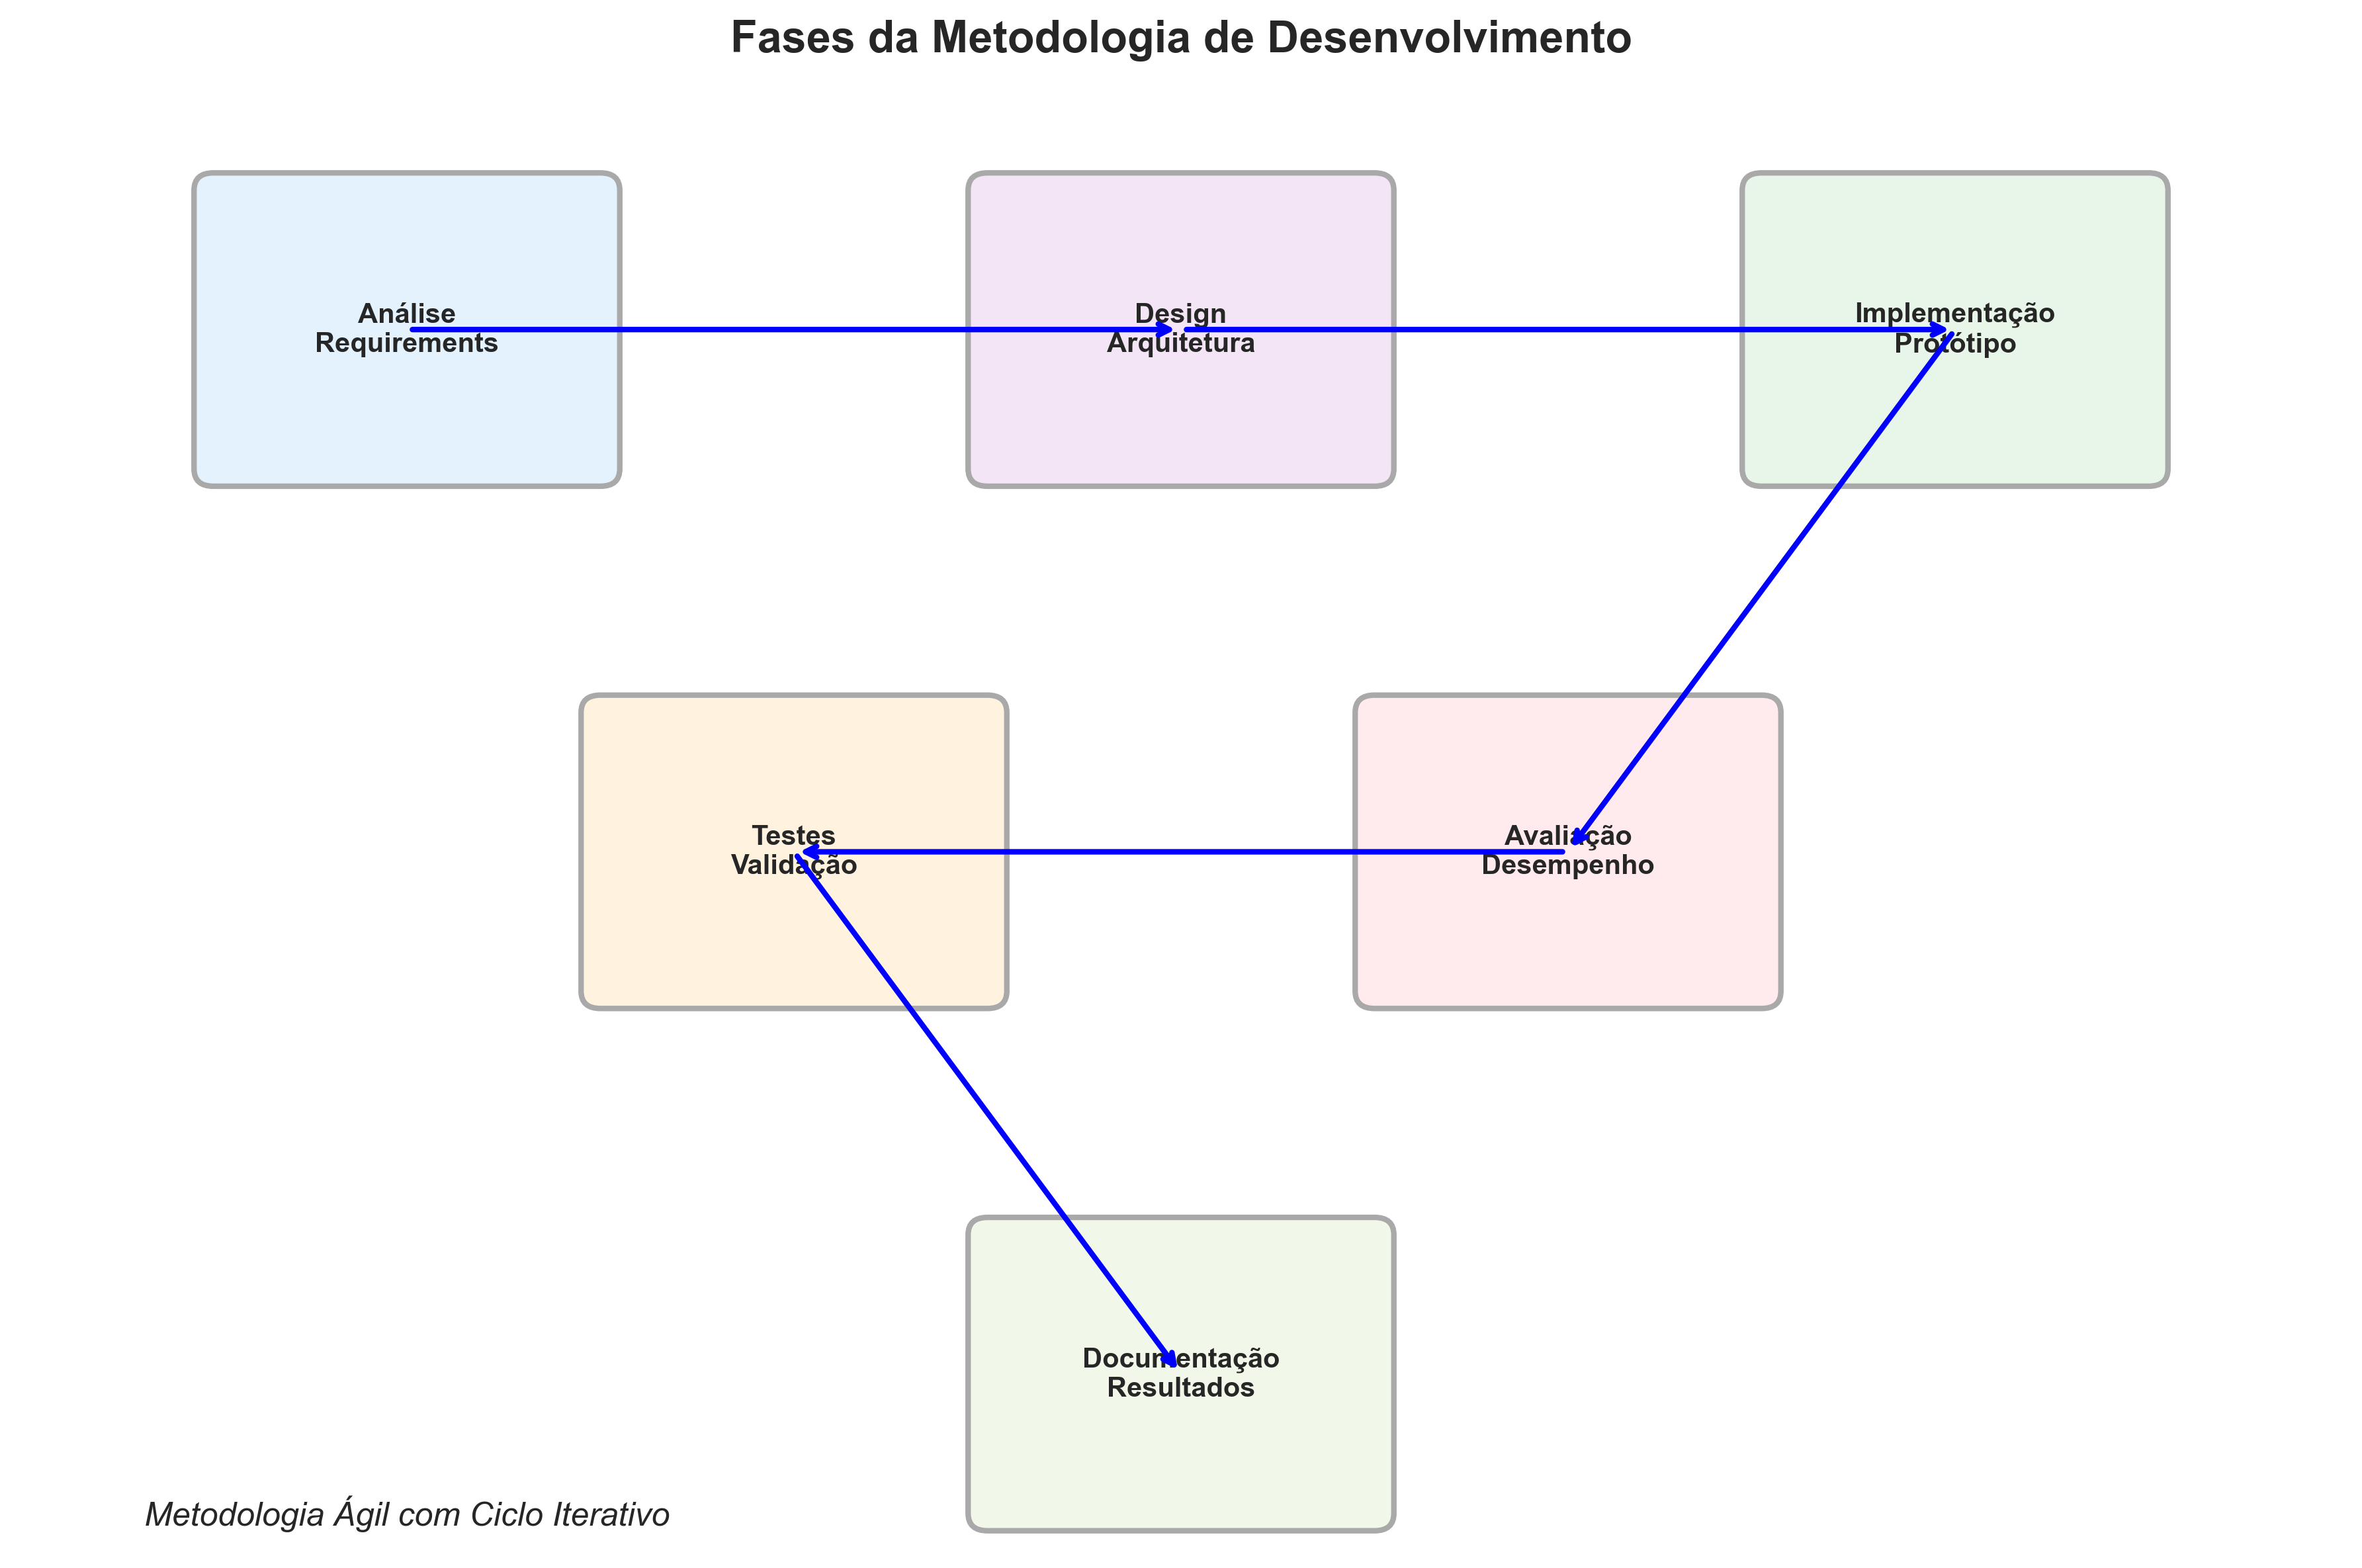
\includegraphics[width=0.9\textwidth]{images/generated/methodology_phases.png}
    \caption{Fases da investigação e metodologia de desenvolvimento do sistema de gestão medicamentosa.}
    \label{fig:methodology_phases}
\end{figure}

\textbf{Fase 1: Análise e Diagnóstico}
- Revisão sistemática da literatura
- Análise dos processos atuais na SCMVV
- Identificação de requisitos funcionais e não-funcionais

\textbf{Fase 2: Conceção e Prototipagem}
- Desenvolvimento de protótipos funcionais
- Validação com profissionais de saúde
- Refinamento iterativo dos requisitos

\textbf{Fase 3: Implementação e Testes}
- Desenvolvimento do sistema final
- Testes de funcionalidade e usabilidade
- Validação em ambiente controlado

\textbf{Fase 4: Avaliação e Validação}
- Implementação piloto na SCMVV
- Recolha de dados de desempenho
- Análise de resultados e impacto

\section{Métodos de Recolha de Dados}

\subsection{Dados Quantitativos}

\textbf{Métricas de Performance:}
- Tempo de resposta do sistema
- Taxa de erros de medicação
- Eficiência dos processos (tempo de prescrição, validação, administração)
- Disponibilidade do sistema

\textbf{Métricas de Utilização:}
- Número de utilizadores ativos
- Frequência de utilização por módulo
- Padrões de navegação e interação

\subsection{Dados Qualitativos}

\textbf{Entrevistas Semiestruturadas:}
- Profissionais de saúde (médicos, enfermeiros, farmacêuticos)
- Gestores hospitalares
- Administradores de sistemas

\textbf{Observação Participante:}
- Observação de processos de trabalho
- Identificação de dificuldades e oportunidades
- Avaliação da integração do sistema nos workflows existentes

\section{Critérios de Avaliação}

\subsection{Critérios de Eficácia}

\textbf{Segurança do Paciente:}
- Redução de erros de medicação \cite{ciapponi2021}
- Melhoria na rastreabilidade de medicamentos
- Redução de eventos adversos

\textbf{Eficiência Operacional:}
- Redução do tempo de processos
- Melhoria na comunicação interdisciplinar
- Otimização da utilização de recursos

\subsection{Critérios de Aceitação}

\textbf{Usabilidade:}
- Facilidade de utilização (System Usability Scale)
- Satisfação dos utilizadores
- Tempo de aprendizagem

\textbf{Adoção:}
- Taxa de adoção por categoria profissional
- Frequência de utilização
- Resistência à mudança \cite{venkatesh2003}

\section{Validação e Verificação}

\subsection{Validação Funcional}

O sistema é validado através de:
- Testes de funcionalidade em ambiente controlado
- Verificação de conformidade com requisitos clínicos
- Validação de integrações com sistemas existentes

\subsection{Validação Clínica}

\textbf{Estudo Piloto:}
- Implementação controlada em serviço específico
- Comparação com processos manuais existentes
- Análise de impacto na segurança do paciente

\textbf{Critérios de Sucesso:}
- Redução mensurável de erros de medicação
- Aceitação positiva pelos profissionais de saúde
- Melhoria dos indicadores de qualidade hospitalar

\section{Considerações Éticas}

\subsection{Proteção de Dados}

O estudo cumpre rigorosamente os requisitos do RGPD \cite{european2016}, garantindo:
- Anonimização de dados de pacientes
- Consentimento informado dos profissionais participantes
- Segurança e confidencialidade das informações

\subsection{Aprovação Ética}

O projeto foi submetido e aprovado pela Comissão de Ética da SCMVV, cumprindo todos os requisitos éticos para investigação envolvendo dados de saúde.

\section{Limitações do Estudo}

\subsection{Limitações Metodológicas}

- Estudo limitado a um único centro hospitalar
- Período de observação limitado a 6 meses
- Possível viés de seleção dos participantes

\subsection{Limitações Técnicas}

- Integração limitada com sistemas externos
- Dependência de infraestrutura existente
- Restrições de recursos computacionais

\section{Cronograma de Execução}

\begin{figure}[htbp]
    \centering
    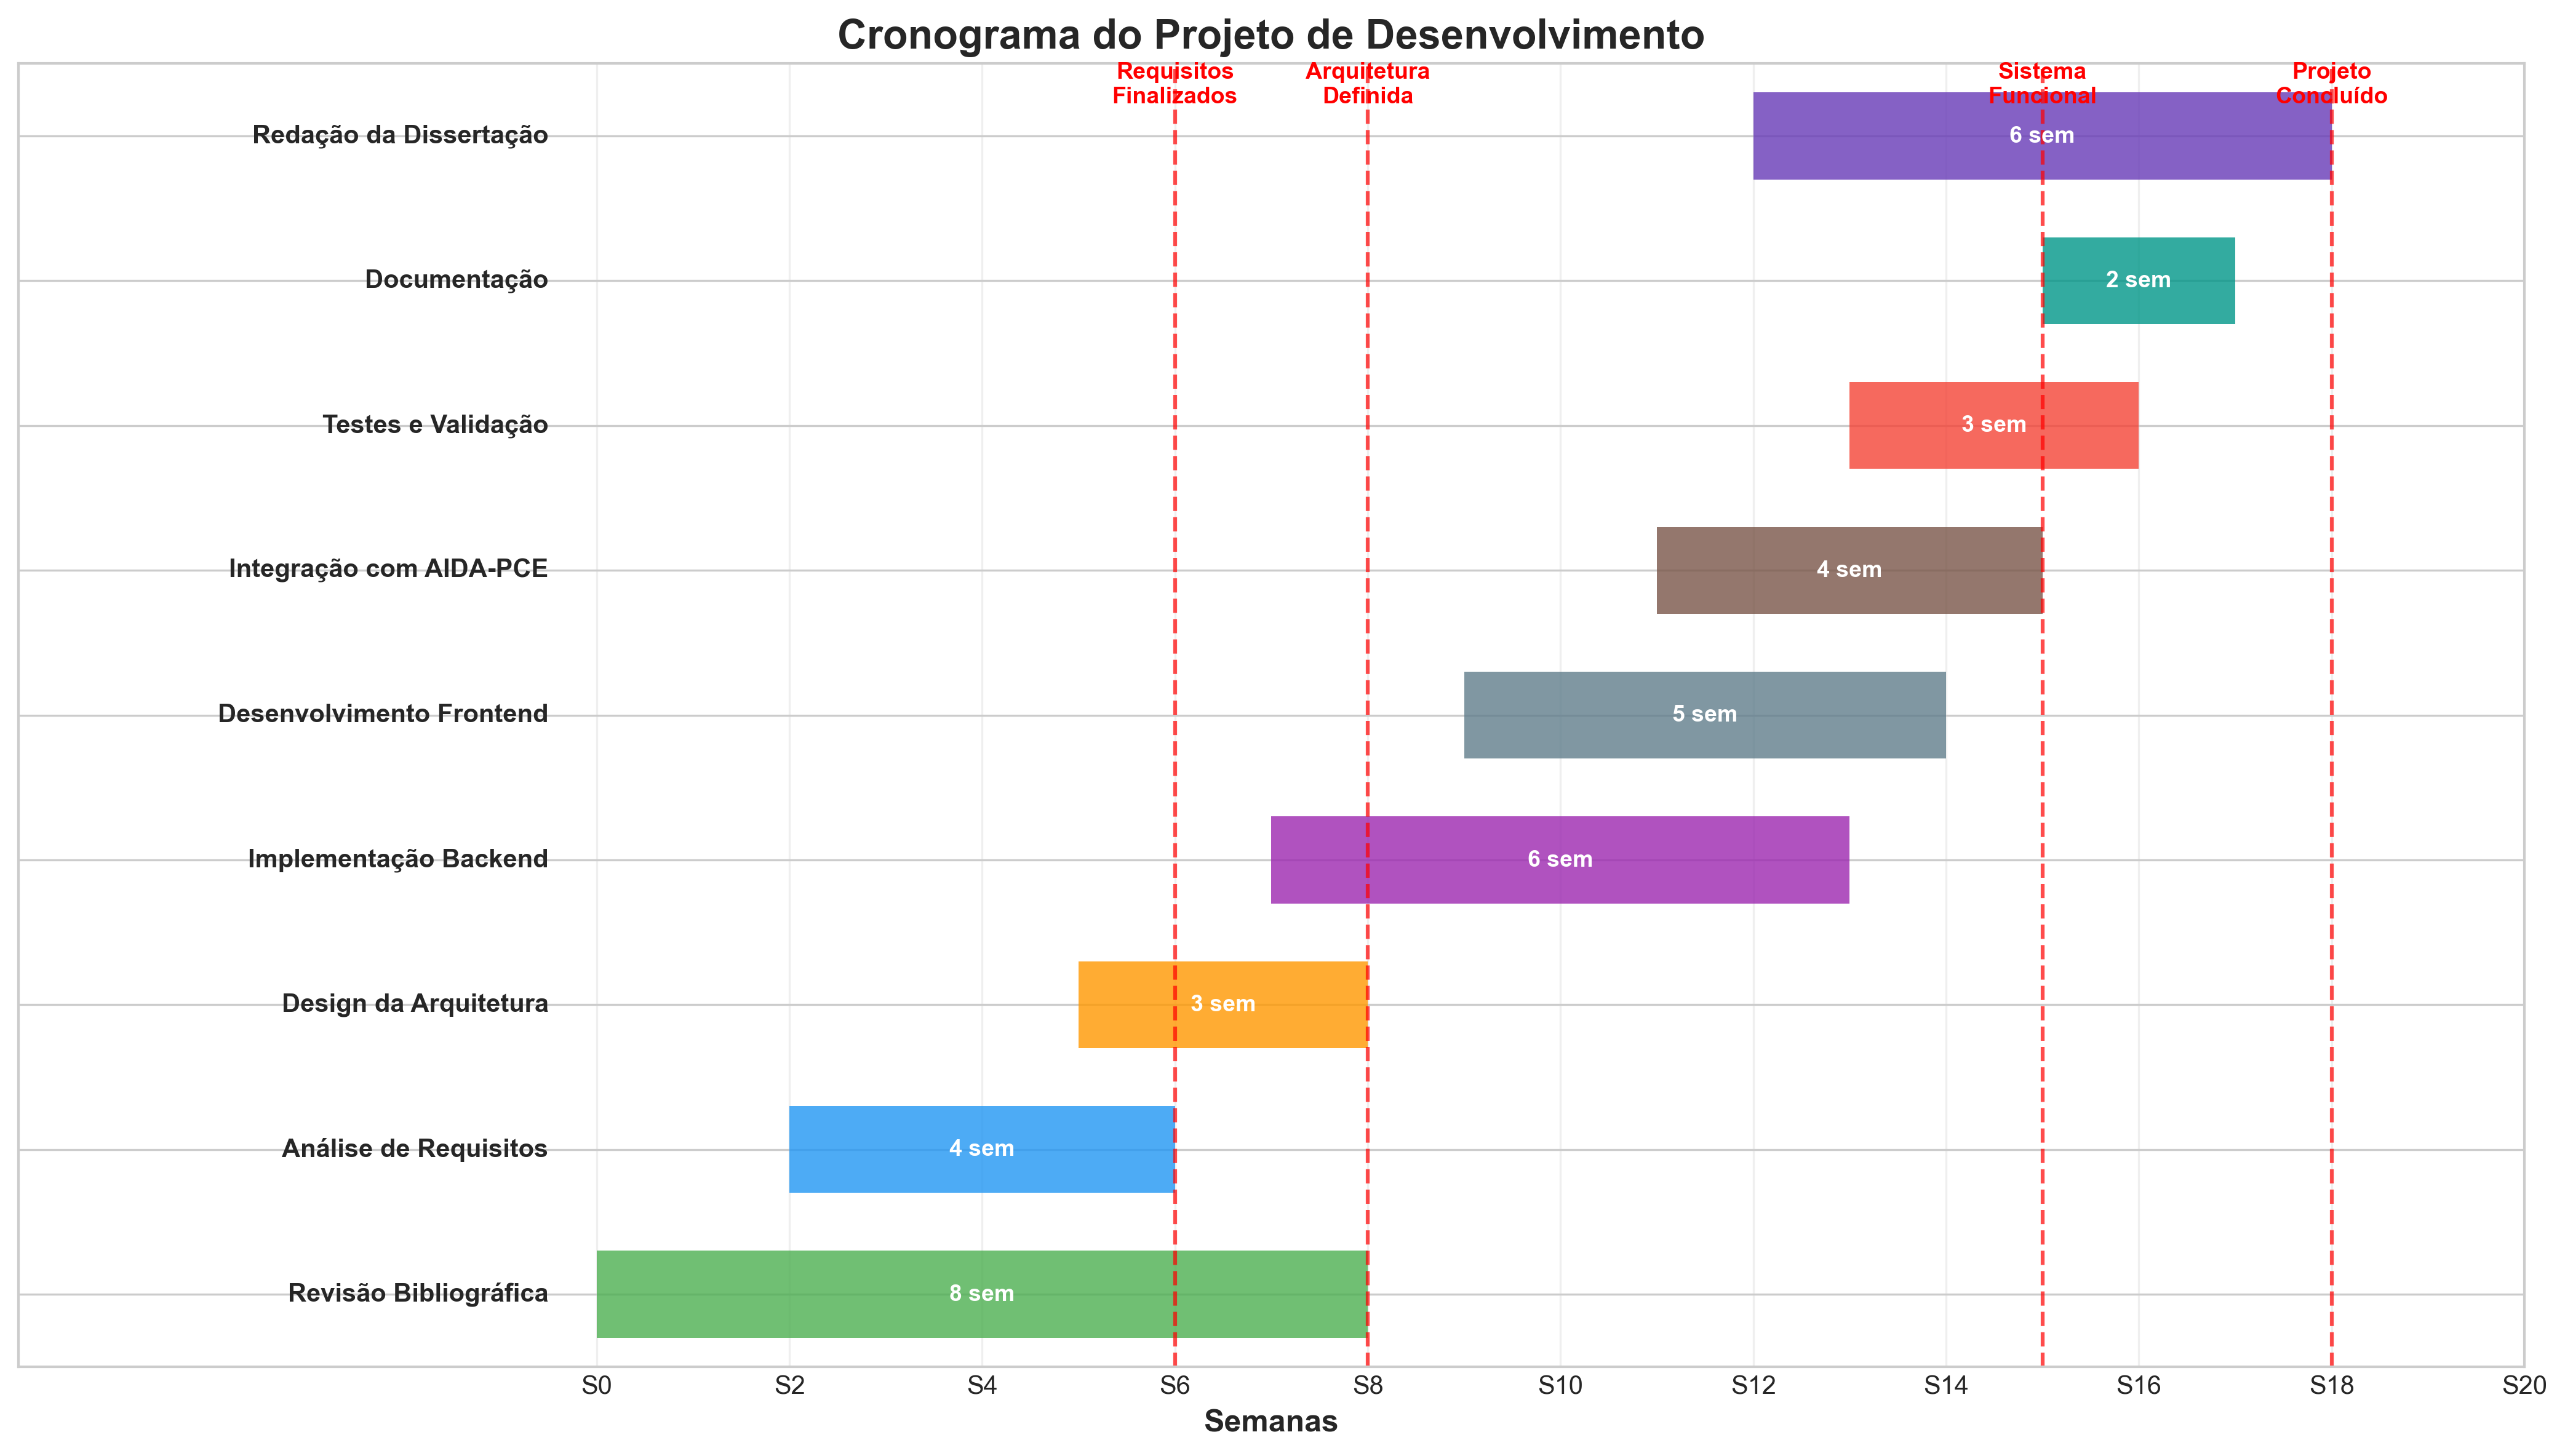
\includegraphics[width=0.95\textwidth]{images/generated/project_timeline.png}
    \caption{Cronograma de execução do projeto de investigação, mostrando as principais fases e marcos.}
    \label{fig:project-timeline}
\end{figure}

O projeto segue um cronograma rigoroso distribuído por 12 meses, com marcos bem definidos e pontos de avaliação contínua. Cada fase inclui objetivos específicos, deliverables e critérios de sucesso claramente estabelecidos. 